\documentclass[12pt]{article}
\usepackage{graphicx,import}
\usepackage[svgnames]{xcolor} 
\usepackage{fancyhdr}
\usepackage{subfig}
\usepackage{hyperref}
\usepackage{enumitem}
\usepackage{cite}
\usepackage[many]{tcolorbox}
\usepackage{listings }
\usepackage[a4paper, total={6in, 8in} , bottom = 25mm , top = 25mm, headheight = 1.25cm , includehead,includefoot,heightrounded ]{geometry}
\usepackage{afterpage}
\usepackage{amssymb}
\usepackage{fancyvrb}
\usepackage{pdflscape}
\usepackage{gensymb}
\usepackage{textcomp}
\usepackage{xecolor}
\usepackage{rotating}
\usepackage{pdfpages}
\usepackage[Kashida]{xepersian}
\usepackage[T1]{fontenc}
\usepackage{tikz}
\usepackage[utf8]{inputenc}
\usepackage{PTSerif} 
\usepackage{seqsplit}

\usepackage[edges]{forest}

\usepackage{listings}
\usepackage{xcolor}

\hypersetup{
	colorlinks   = true, %Colours links instead of ugly boxes
	urlcolor     = blue, %Colour for external hyperlinks
	linkcolor    = blue, %Colour of internal links
	citecolor   = red %Colour of citations
}
 
\definecolor{codegreen}{rgb}{0,0.6,0}
\definecolor{codegray}{rgb}{0.5,0.5,0.5}
\definecolor{codepurple}{rgb}{0.58,0,0.82}
\definecolor{backcolour}{rgb}{0.95,0.95,0.92}
 
\NewDocumentCommand{\codeword}{v}{
\texttt{\textcolor{blue}{#1}}
}
\lstset{language=java,keywordstyle={\bfseries \color{blue}}}

\lstdefinestyle{mystyle}{
    backgroundcolor=\color{backcolour},   
    commentstyle=\color{codegreen},
    keywordstyle=\color{magenta},
    numberstyle=\tiny\color{codegray},
    stringstyle=\color{codepurple},
    basicstyle=\ttfamily\normalsize,
    breakatwhitespace=false,         
    breaklines=true,                 
    captionpos=b,                    
    keepspaces=true,                 
    numbers=left,                    
    numbersep=5pt,                  
    showspaces=false,                
    showstringspaces=false,
    showtabs=false,                  
    tabsize=2
}

\lstset{style=mystyle}

\settextfont[Scale=1.2 ,BoldFont={Bahij Nazanin-Bold.ttf} , ItalicFont = {IRNazaninIranic.ttf}]{Bahij Nazanin-Regular.ttf}
\setlatintextfont[Scale = 1.0]{Garamond}
\DefaultMathsDigits 
\DeclareMathSizes{11}{19}{13}{9} 
%\DeclareMathSizes{12}{14.4}{8}{9}





\newenvironment{changemargin}[2]{%
\begin{list}{}{%
\setlength{\topsep}{0pt}%
\setlength{\leftmargin}{#1}%
\setlength{\rightmargin}{#2}%
\setlength{\listparindent}{\parindent}%
\setlength{\itemindent}{\parindent}%
\setlength{\parsep}{\parskip}%
}%
\item[]}{\end{list}}


\definecolor{foldercolor}{RGB}{124,166,198}

\tikzset{pics/folder/.style={code={%
    \node[inner sep=0pt, minimum size=#1](-foldericon){};
    \node[folder style, inner sep=0pt, minimum width=0.3*#1, minimum height=0.6*#1, above right, xshift=0.05*#1] at (-foldericon.west){};
    \node[folder style, inner sep=0pt, minimum size=#1] at (-foldericon.center){};}
    },
    pics/folder/.default={20pt},
    folder style/.style={draw=foldercolor!80!black,top color=foldercolor!40,bottom color=foldercolor}
}

\forestset{is file/.style={edge path'/.expanded={%
        ([xshift=\forestregister{folder indent}]!u.parent anchor) |- (.child anchor)},
        inner sep=1pt},
    this folder size/.style={edge path'/.expanded={%
        ([xshift=\forestregister{folder indent}]!u.parent anchor) |- (.child anchor) pic[solid]{folder=#1}}, inner xsep=0.6*#1},
    folder tree indent/.style={before computing xy={l=#1}},
    folder icons/.style={folder, this folder size=#1, folder tree indent=3*#1},
    folder icons/.default={12pt},
}

\begin{document}


%%% title pages
\begin{titlepage}
\begin{center}
        
\vspace*{0.7cm}


\includegraphics[width=0.4\textwidth]{sharif1.png}\\
\vspace{0.5cm}
\textbf{ \Huge{\emph ‌اندازه‌گیری و کنترل کامپیوتری} }\\
\vspace{0.5cm}
\textbf{ \Large{ تمرین هفتم} }
\vspace{0.2cm}
       
 
      \large \textbf{دانشکده مهندسی کامپیوتر}\\\vspace{0.2cm}
    \large   دانشگاه صنعتی شریف\\\vspace{0.2cm}
       \large   ﻧﯿﻢ سال دوم 00-99 \\\vspace{0.2cm}
      \noindent\rule[1ex]{\linewidth}{1pt}
استاد:\\
    \textbf{{جناب آقای دکتر همت‌یار}}


    \vspace{0.15cm}
نام و نام خانوادگی:\\

       
    \textbf{{امیرمهدی نامجو - 97107212}}
\end{center}
\end{titlepage}
%%% title pages


%%% header of pages
\newpage
\pagestyle{fancy}
\fancyhf{}
\fancyfoot{}
\cfoot{\thepage}
\chead{تمرین هفتم}
\rhead{
\includegraphics[width=0.1\textwidth]{sharif.png}}
\lhead{امیرمهدی نامجو}
%%% header of pages

\KashidaOff


\section*{سوال 7}

\begin{enumerate}
	\item 

دیود زنر به جز در مواقع لحظه های کوتاهی که ولتاژ صفر می‌شود، $5.1$ ولت را تامین می کند. دوره تناوب بخش مثبت نمودار هم
$1/(60*2)=1/120 s$
است. با توجه به این موضوع داریم:

$$V_c =5.1 (1 - e^{-t / \tau})$$

$$1.5 = 5.1(1 - e^{-t/\tau}) $$

$$t/\tau = -\ln (1 - 1.5 /5.1) = 0.348$$

$$t= 0.348 \tau = 0.348 (R_T + R)C$$

برای زمان روشنایی $10$ درصد، عملا باید زمان رسیدن به $1.5$ ولت، به اندازه $90$ درصد دوره تناوب طول بکشد و برای زمان روشنایی $90$ درصد، باید زمان رسیدن به $1.5$ ولت، $10$ درصد تناوب طول بکشد.

پس برای $0$ درجه، باید به
$0.9 \times 1/120 = 7.5 ms$
و برای
$60$ درجه
به
$0.1 \times 1/120 = 0.83 ms$
برسیم.

طبق جداول فصل $4$ و مقاومت های ترمیستور در دمای $0$ مقاومت $16 k\Omega$ و در $60$ مقاومت $1k\Omega$ است. پس داریم:

$$0.0075 = 0.348(16000  + R)C$$
$$0.00083 = 0.348(1000+R)C$$

با حل معادلات داریم:

$$R\approx 875 \Omega , C \approx 1.28 \mu F$$

\item

برای محاسبه توان، ابتدا باید ولتاژ میانگین منبع تغذیه را بدست آوریم:

$$\frac{1}{T}\int_{0}^{T} V_0 sin(2 \pi \times 60 t) dt$$

که در آن $T$ با توجه به \lr{full-wave rectified} بودن مدار به خاطر پل دیودها و این که تناوب مثبت را می‌خواهیم برابر $1/120$ است. و همچنین $V_0 =120 \sqrt{2}$ است. با محاسبه انتگارل داریم:

$$\bar{V} = \frac{240 \sqrt{2}}{\pi } = 108.4 V$$

در نتیجه توان اتقالی در مقاومت برابر خواهد بود با:
$$P_R =(108.4-5.1)^2 / (2500) = 4.27 W$$

پس مقاومت باید حدودا تحمل $5$ وات را داشته باشد.

جریان گذرنده از زنر همان جریان گذرنده از مقاومت است.
$$I = (108.4-5.1)/2500 = 0.041A$$

پس توان اتلاقی در زنر:

$$P_Z =0.041\times 5.1 = 0.21 W$$
است. پس یک زنر نیم واتی هم کافی خواهد بود.

\item

عملا ولتاژ میانگین دو سر موتور به صورت زیر می شود:
$$\frac{1}{T}\int_{t}^{T} V_0 sin(2 \pi \times 60 t) dt = \frac{120 \sqrt{2} (\cos (120 \pi  t)+1)}{\pi }$$

و از طرفی داریم که 
$$t = 0.348 (R_T + 875)(1.28 \times 10^{-6})$$ 

با جایگذاری نهایی چنین فرمولی برحسب مقاومت بدست می‌آید:

$$V \approx 54(1+\cos(1.68 \times 10^{-4}(R_T + 875)))$$

اگر نمودار را برحسب $R$ رسم کنیم، به چنین شکلی میرسیم:

\begin{center}
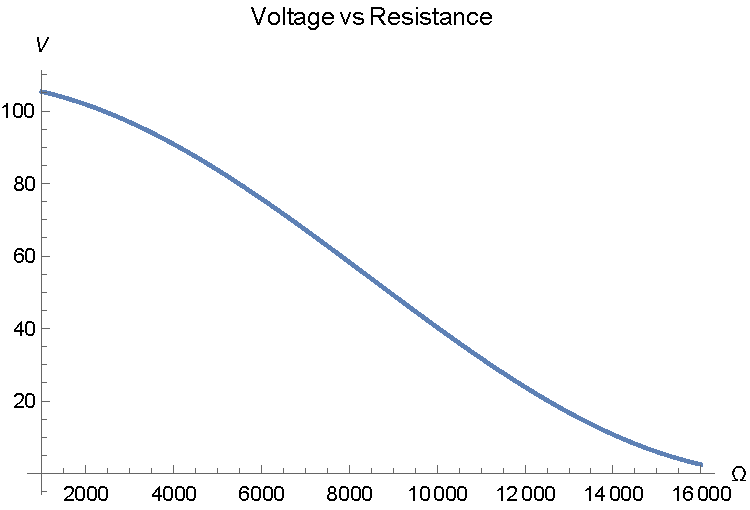
\includegraphics[width =0.5\textwidth]{images/1.pdf}	
\end{center}

اما سوال برحسب دما خواسته است. با بدست آوردن رابطه دما با مقاومت برحسب نمودارهای فصل ۴، به جدول زیر می رسیم:

$$
\begin{array}{|l|l|l|}
	\hline \text { Temperature }\left({ }^{\circ} \mathrm{C}\right) & \text { Resistance }(\mathrm{k} \Omega) & \text { Voltage (V) } \\
	\hline 0 & 16 & 2.5 \\
	\hline 10 & 10 & 40.3 \\
	\hline 20 & 6.5 & 71.6 \\
	\hline 30 & 4.5 & 87.4 \\
	\hline 40 & 3 & 97.0 \\
	\hline 50 & 2 & 101.8 \\
	\hline 60 & 1 & 105.3 \\
	\hline
\end{array}
$$

و با رسم این داده‌ها برحسب دما به چنین نموداری (ولتاژ برحسب دما) می‌رسیم:

\begin{center}
	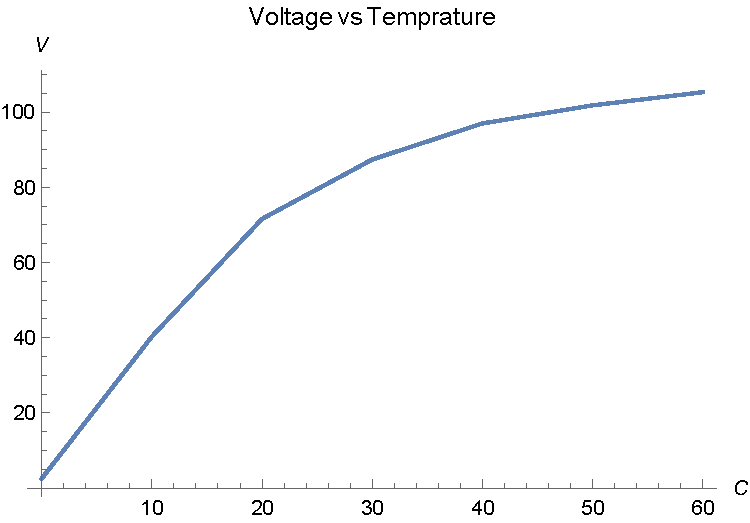
\includegraphics[width =0.5\textwidth]{images/2.pdf}
\end{center}


\end{enumerate}

 
 
\end{document}



